\documentclass[spanish, a4paper, 12pt] {article}
\usepackage[spanish]{babel}
\usepackage[utf8]{inputenc}
\usepackage{amsmath}
\usepackage{amssymb}
\usepackage{amsfonts}
\usepackage{latexsym}
\usepackage{mathtools}
\usepackage{anysize}
%\marginsize{2cm}{2cm}{2cm}{3cm}
\newcommand\eqdef{\stackrel{\mathclap{\mbox{\tiny{def}}}}{=}}
\newcommand\eqac{\stackrel{\mathclap{\mbox{*}}}{=}}

\usepackage{graphicx}
\usepackage{hyperref}
\usepackage{float}
\usepackage{verbatim}
\DeclareGraphicsExtensions{.pdf,.png,.jpg}

\usepackage[a4paper,bindingoffset=0.2in,left=0.8in,right=0.8in,top=1.1in,bottom=1in,footskip=.25in]{geometry}

\begin{document}
\title{\vspace{-1.75cm}Entrega 2}
\author{Marco Antonio Garrido Rojo\thanks{\url{https://github.com/MaSteve/EDIF} Esta entrega puede encontrarse en GitHub.}\vspace{-0.5cm}}
\date{\vspace{-0.5cm}}
\maketitle
\vspace{-0.25cm}
Sea el sistema no lineal
$\begin{cases}
    x' = f(x, y) = x - y + \frac{xy - x^3 - xy^2}{\sqrt{x^2 + y^2}} \\
    y' = g(x, y) = x + y - \frac{x^2 + x^2y + y^3}{\sqrt{x^2 + y^2}}
\end{cases}$
definido en el abiero $\Omega = \mathbb{R}^2 \backslash \{(0,0)\}$
\begin{itemize}
\item{
\textbf{Apartado A} Comprueba que $(1, 0)$ es un punto de equilibrio del sistema.

Fácil y sencillo, para ver que es un punto de equilibrio basta sustituirlo en el sistema y ver que obtenemos cero en ambas componente.

Tenemos que $f(1,0) = 1 - 0 - 1 = 0$ y $g(1, 0) = 1 + 0 - 1 = 0$, luego ya está.

$\hfill \square$
}
\item{
\textbf{Apartado B} Haz el cambio a polares para determinar todos los puntos de equilibrio del sistema.

El paso a coordenadas polares es el mejor lugar para equivocarse y que luego no salga nada bien en lo que queda de ejercicio. Vamos a ver que podemos hacer:
$$
r' = \frac{xx' + yy'}{r} = \frac{x^2-yx}{r} + \frac{x^2y - x^4 - x^2y^2}{r^2} + \frac{yx + y^2}{r} - \frac{x^2y + x^2y^2 + y^4}{r^2}
$$
Agrupando las fracciones con mismo denominador y sustituyendo $r^2 = x^2 + y^2$, sacamos $\boxed{r' = r(1-r)}$.
$$
\theta' = \frac{y'x - yx'}{r^2} = \frac{x^2+xy}{r^2} - \frac{x^3 + x^3y + y^3x}{r^3} - \frac{xy - y^2}{r^2} - \frac{xy^2 - x^3y - xy^3}{r^3}
$$
Volvemos a usar la misma estrategia de antes y llegamos a $\boxed{\theta' = 1 - \frac{x}{r} = 1 - \cos(\theta)}$, usando que $x = r\cos(\theta)$.

Una vez llegados a este punto, podemos buscar los puntos de equilibrio del nuevo sistema que por la primera ecuación se encuentran a una distancia de $1$ del origen, y por la segunda, únicamente se puede encontrar para $\theta = 0$, con lo que llegamos a que el punto del apartado anterior es el único punto de equilibrio en $\Omega$.

$\hfill \square$
}
\item{
\textbf{Apartado C} Sea $C:=\{(x, y) \in \mathbb{R}^2 / x^2 + y^2 = 1\}$ y el vector $\vec{N} = (2x, 2y)$ normal a $C$ en cada punto. Calcula el producto escalar $\langle(f(x, y), g(x, y)), \vec{N}\rangle$ para deducir que la circunferencia contiene dos trayectorias: $C \backslash \{(1,0)\}$ y $(1,0)$. Concluye que $\{(x, y) \in \mathbb{R}^2 / 0 < x^2 + y^2 < 1\}$ es invariante para el sistema.

Que $(1,0)$ es una trayectoria y que está en la circunferencia ya lo sabemos. La gracia está en el resto de la circunferencia.

Vamos a calcular el producto escalar para ver si por el camino surge algo interesante.
$$
\langle(f(x, y), g(x, y)), \vec{N}\rangle = 2x^2 - 2xy + \frac{2x^2y - 2x^4 - 2x^2y^2}{\sqrt{x^2 + y^2}}
+
2xy + 2y^2 - \frac{2x^2y + 2x^2y^2 + 2y^4}{\sqrt{x^2 + y^2}}
$$
Agrupamos y simplificamos un poco para obtener:
$$
\langle(f(x, y), g(x, y)), \vec{N}\rangle = 2(x^2 + y^2) - 2(x^2 + y^2)(\sqrt{x^2 + y^2}) = 2(x^2 + y^2)(1-\sqrt{x^2 + y^2})
$$

Esta expresión se anula por un casual en los puntos de $C$. ¿Qué significa esta ``casualidad''? Pues que el vector normal $\vec{N}$ es perpendicular también a la trayectoria que siguen los puntos en la circunferencia. En otras palabra, los puntos de la circunferencia trazan la propia circunferencia con las soluciones que pasan por ellos y que resuelven el sistema.

La verdad es que este argumento dicho así parece que pende de un hilo, por eso prefiero utiliza el cañón del apartado anterior para justificar este resultado. Como la $r'$ se anula en los puntos con $r = 1$, tenemos que los puntos que caen ahí, es decir los de $C$, mantienen en sus trayectorias el radio constante. Ahora sí que me quedo contento.

Por último, tenemos que el interior del recinto queda invariante porque las soluciones del sistema no se pueden cortar, por tanto no pueden atravesar la circunferencia.

$\hfill \square$
}
\item{
\textbf{Apartado D} Representa el diagrama de fases con pplane para visualizar que $(1, 0)$ no es estable, aunque las soluciones $\varphi(t, X_0)$ cumplen que $\lim_{t\rightarrow\infty}\varphi(t, X_0) = (1,0)$ para todo $X_0 \in \Omega$.

Pues pinta, colorea y analiza.

{\begin{figure}[!ht]
\centering
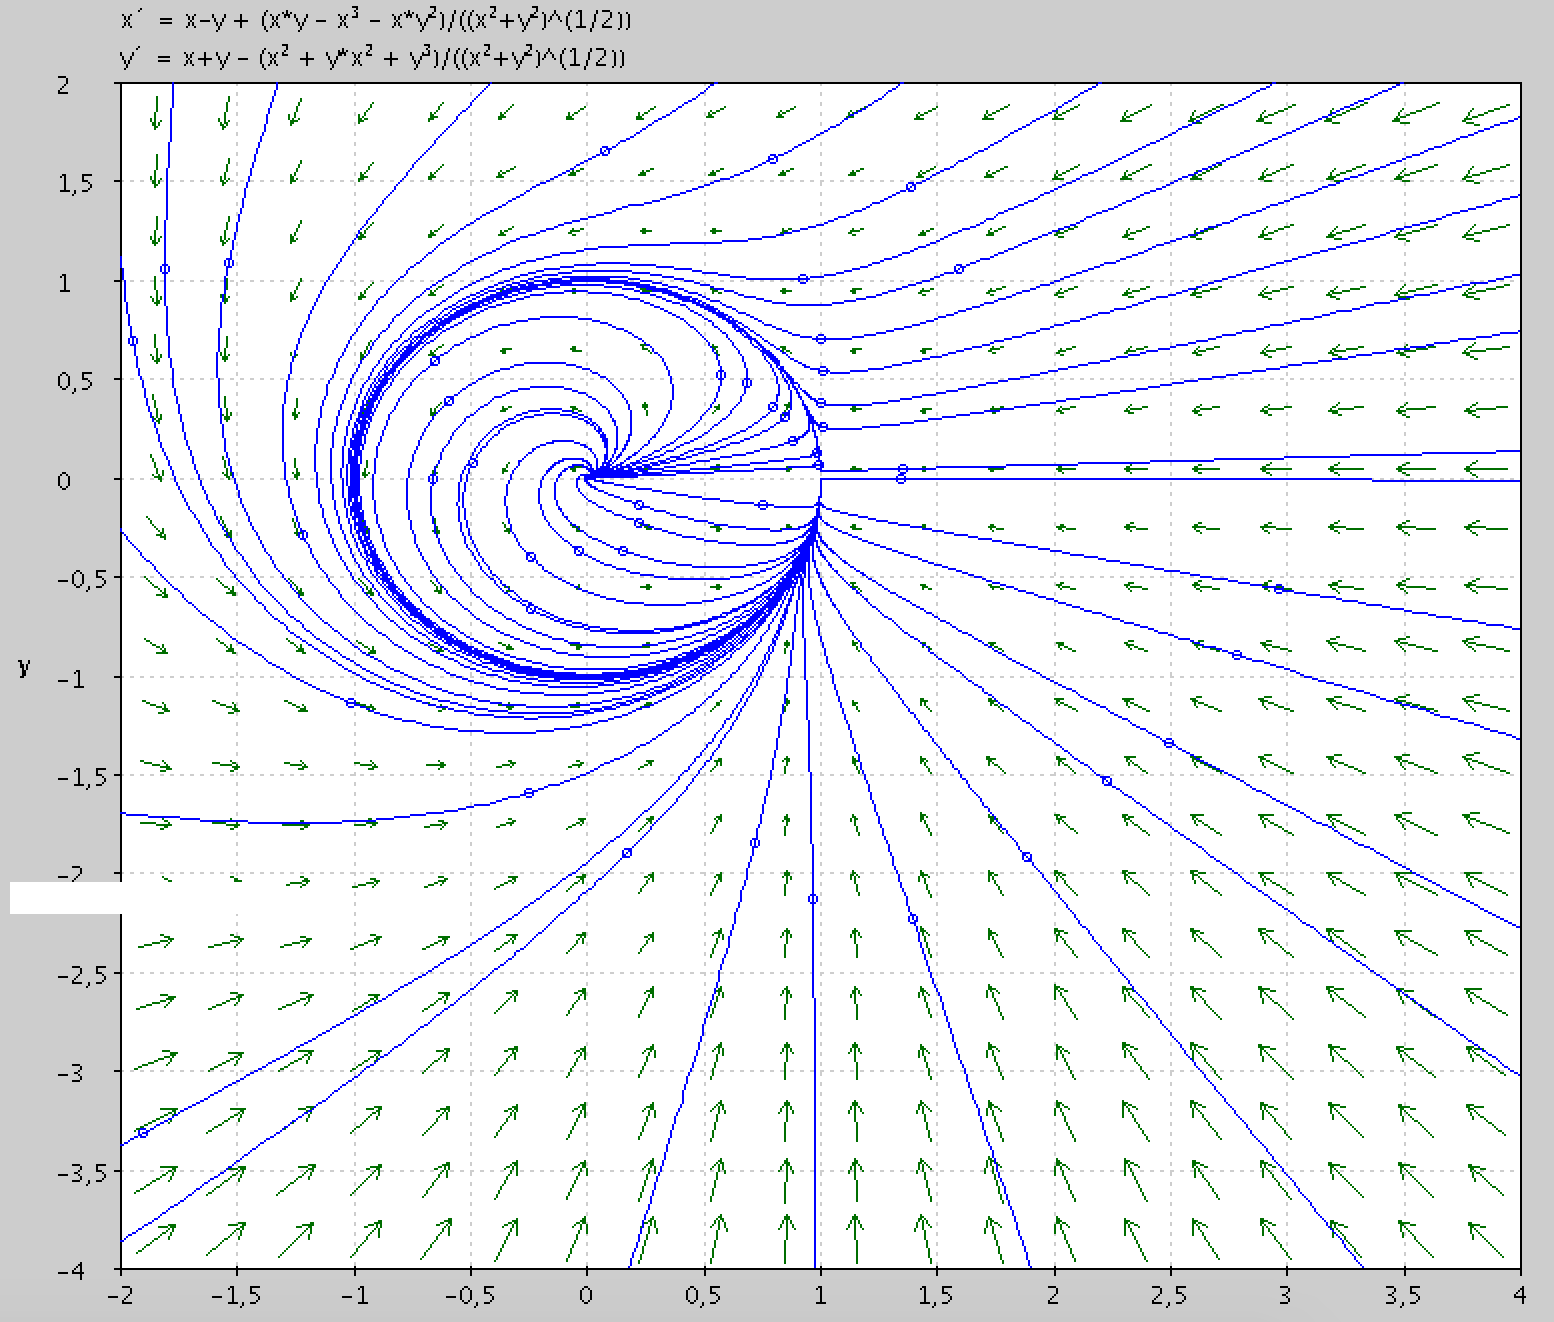
\includegraphics[width=0.4\textwidth]{plot.png}
\caption{Diagrama de fases.}
\end{figure}}

Ya podíamos tener la sospecha de que el punto no iba a ser estable porque tenemos la trayectoria que recorre toda la circunferencia menos el punto $(1,0)$, que sale de este y llega a este. También podríamos habernos dado cuenta de este problema mirando el sistema en polares y fijándonos en la ecuación para la $\theta'$. Para ángulos por encima del eje x tenemos que se aleja, y para valores por debajo del eje x tenemos que se acerca.

$\hfill \square$
}
\end{itemize}
\end{document}
